\mojesekce{Results}

\subsection{Sensitivity analyses}
\begin{block}{Sensitivity analyses}
\justifying
Each optimized parameter were increased and decreased with specific factor unit sum of squares increased with order of magnitude. 
\begin{columns}
    \begin{column}{0.4\textwidth}
        \begin{table}[]
            \begin{tabular}{lll}
                \hline
                \hline
                Paraneter & increase   & decrease \\
                          & factor (+) & factor (-) \\
                \hline
                X         & 80                  & 1/3.5               \\
                Y         & 1.3                 & 1/1.6               \\
                b         & 1.125               & 1/1.5               \\
                Ks        & 2.0                 & 1/5.0               \\
                S         & 2.0                 & 1/5.0               \\
                ret       & 1.5                 & 1/5.0              \\
                \hline
                \hline
            \end{tabular}
        \end{table}
    \end{column}
    \begin{column}{0.6\textwidth}
        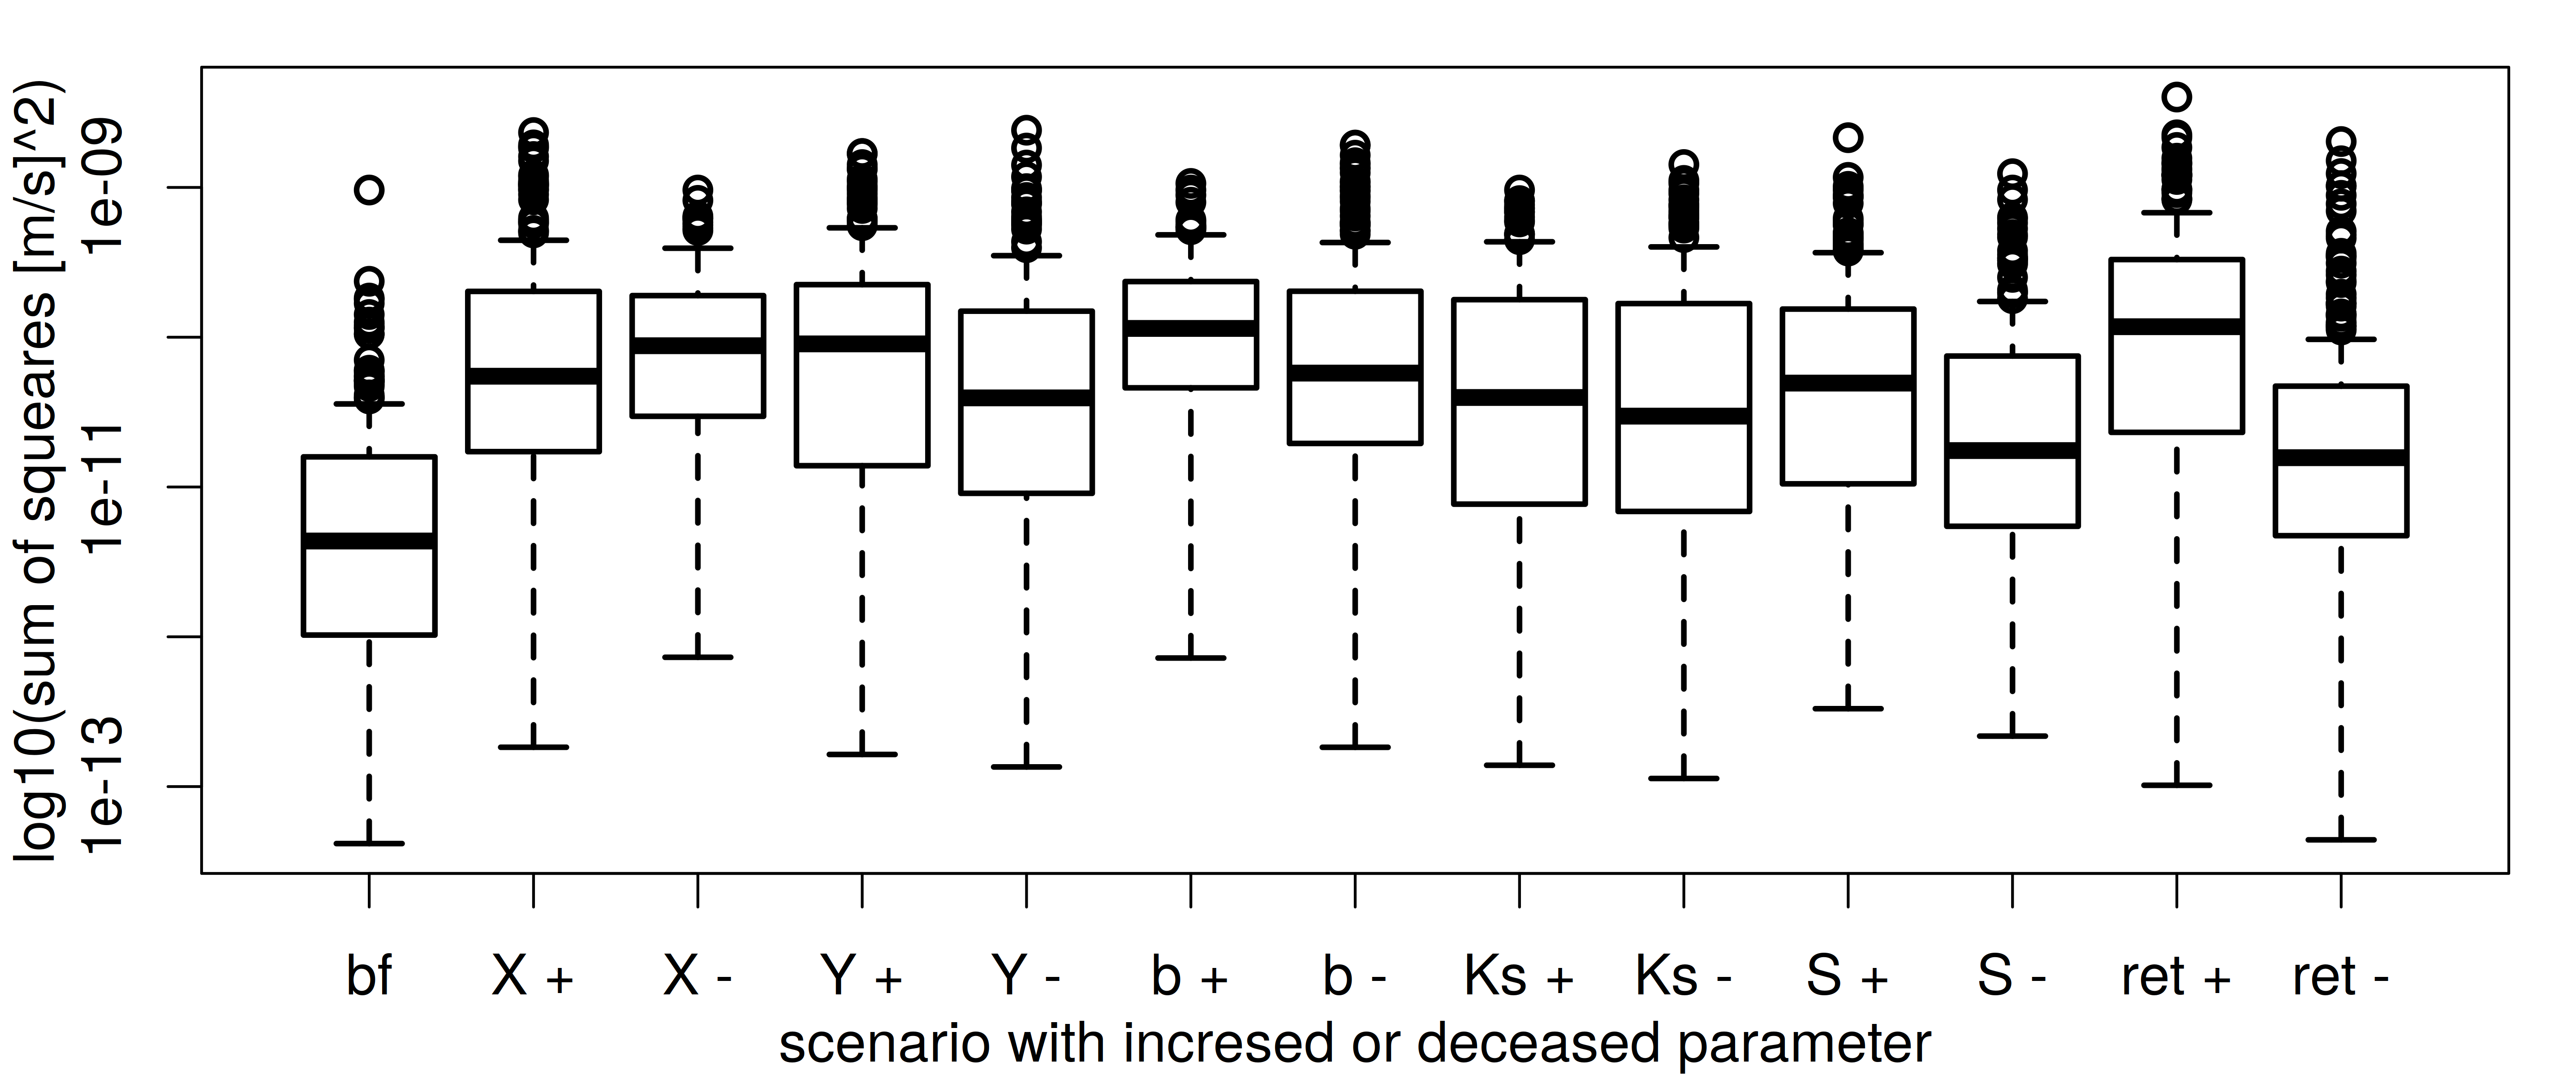
\includegraphics[width = \textwidth]{obr/sens.png}
    \end{column}
\end{columns}
\end{block}


\subsection{Model parameters and textural classes}
\begin{block}{Model parameters and textural classes}
\begin{columns}
    \begin{column}{0.2\textwidth}
    \end{column}
    \begin{column}{0.6\textwidth}

        \begin{table}[]
            \begin{tabular}{lllll}
            parameter: & X & Z & b & ret \\
            max & 30 & 5 & 4 & 0 \\
            min & 1 & 0.01 & 1 & -0.5 \\
            \end{tabular}
        \end{table}
    \end{column}
\end{columns} 

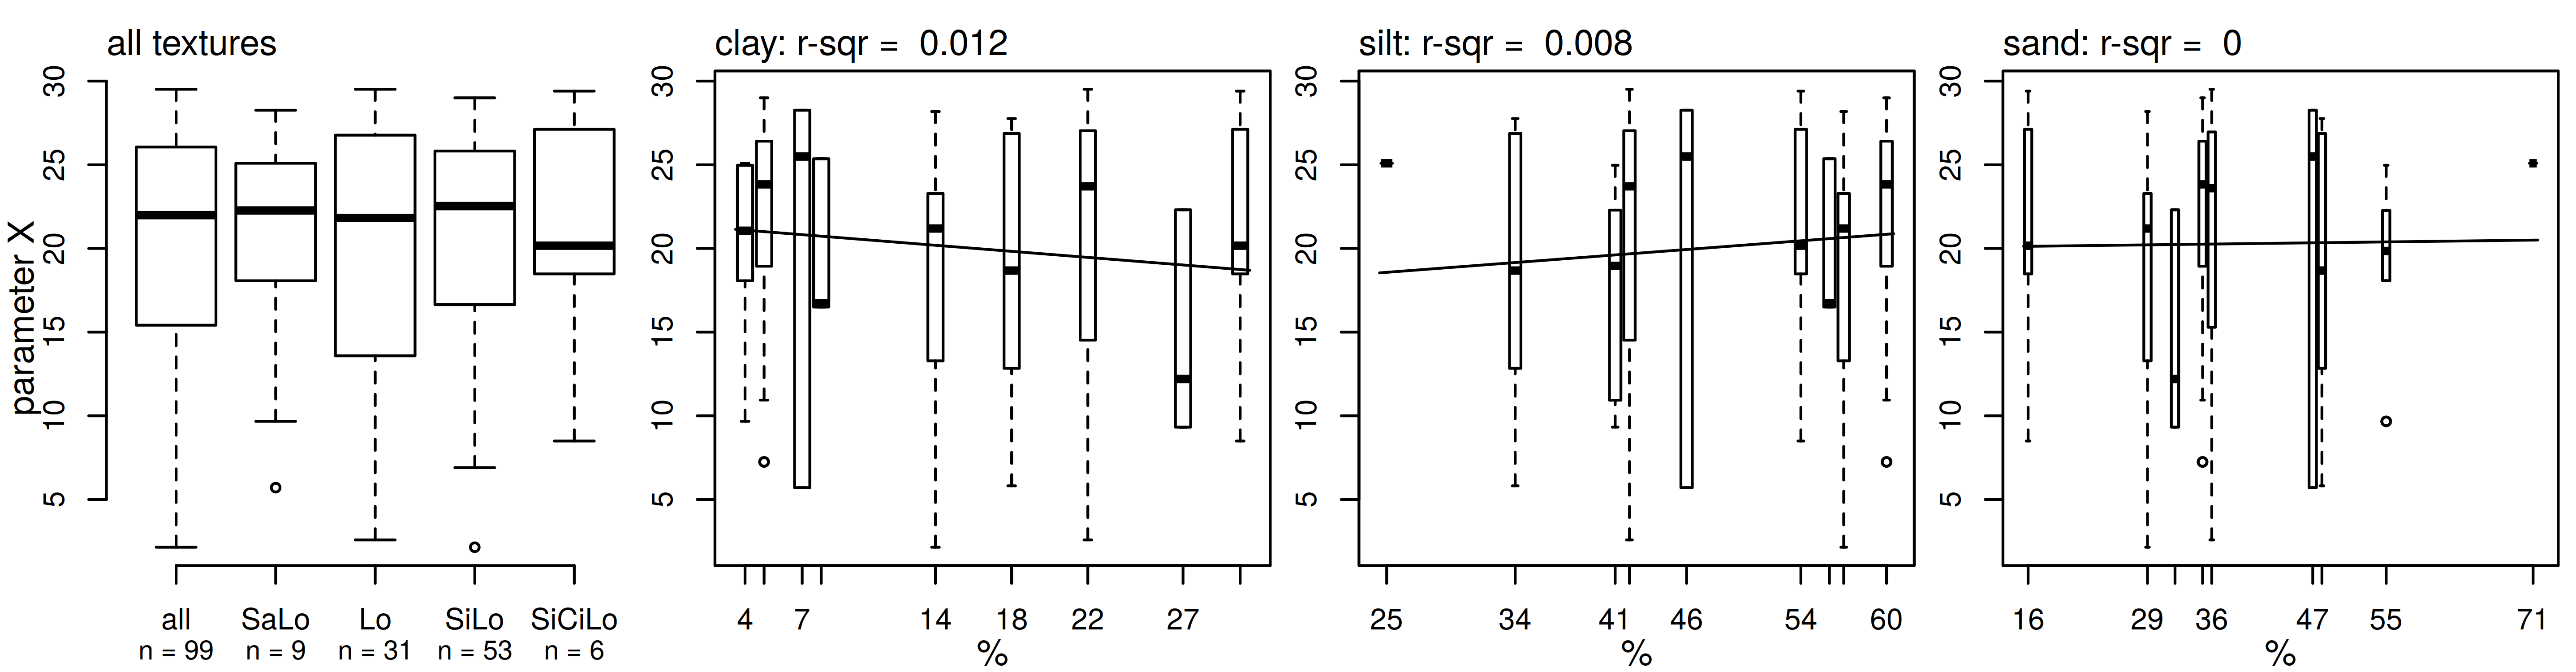
\includegraphics[width = \textwidth]{obr/Xfittex.png}
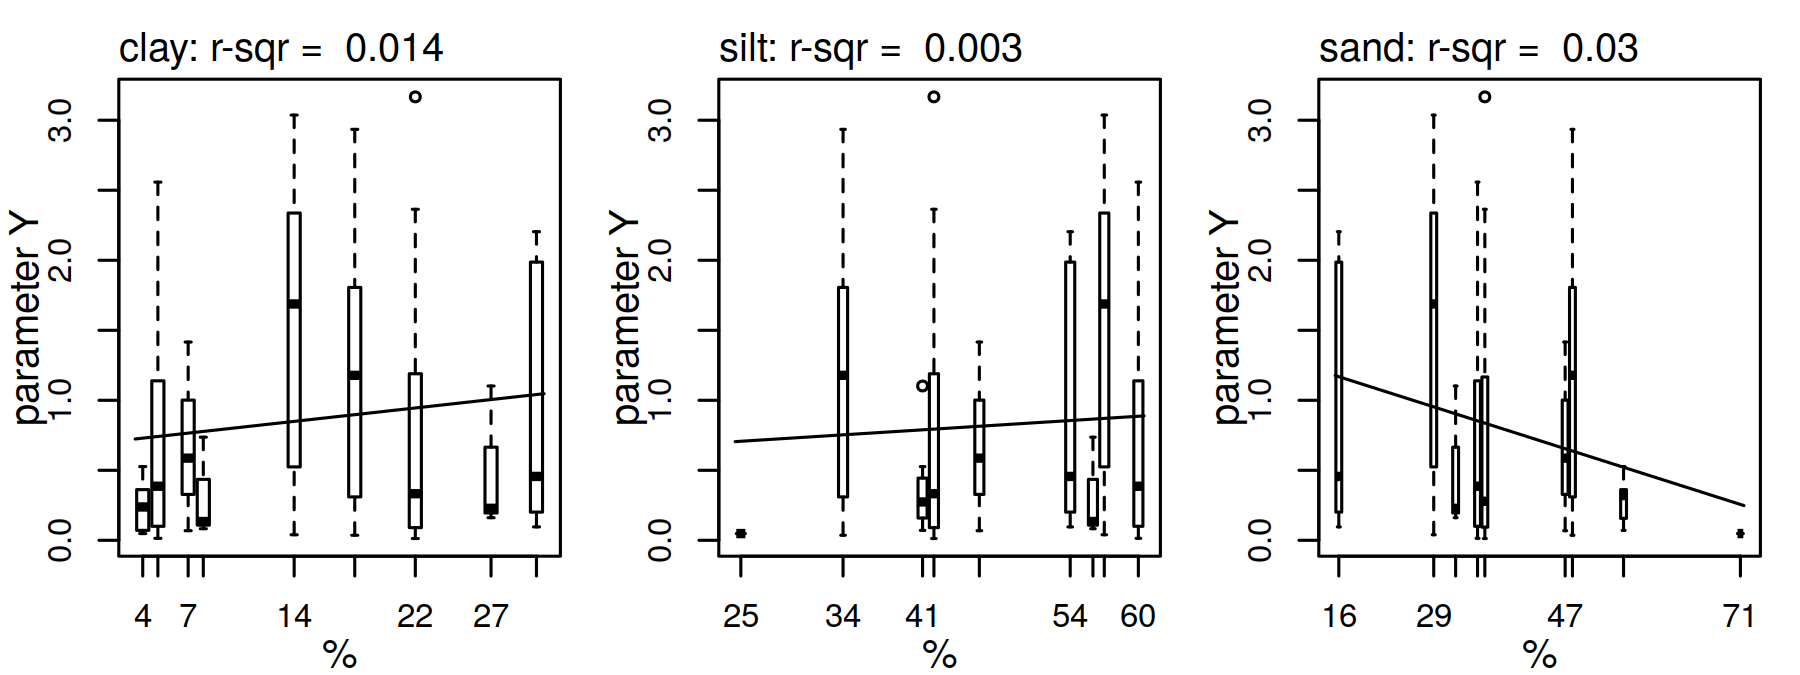
\includegraphics[width = \textwidth]{obr/Yfittex.png}
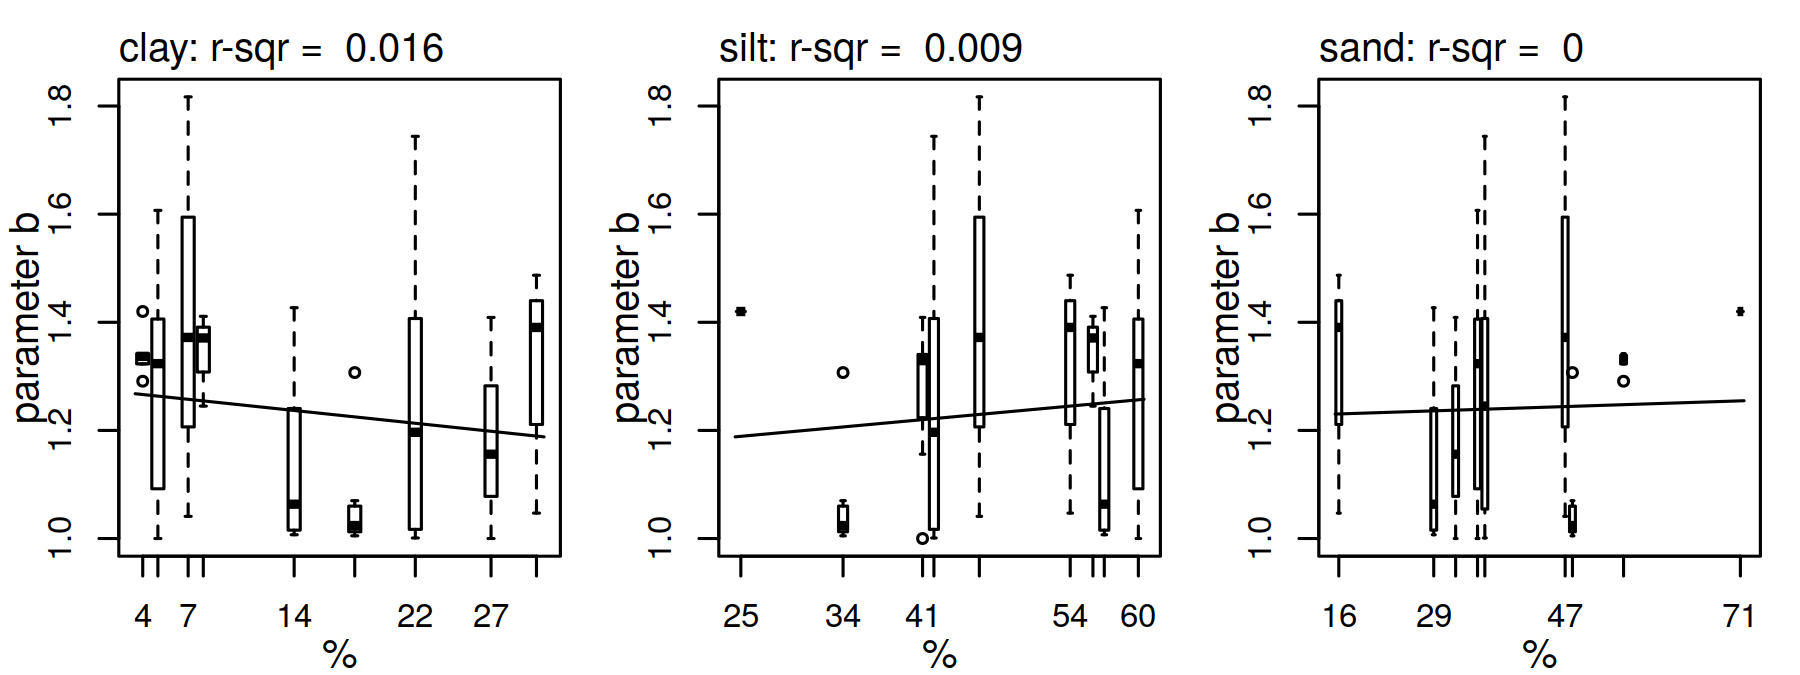
\includegraphics[width = \textwidth]{obr/bfittex.png}
\end{block}


